\documentclass[12pt,a4paper,english]{beamer}
\usepackage{ucs}
\usepackage[utf8x]{inputenc}%utf-8
%\usepackage{lmodern}
\usepackage{fontenc}%[T1]
\usepackage{babel}%[T1]
\usepackage{amssymb,amsmath,wick}
\usepackage{epsfig}
\usepackage{wrapfig}
\usepackage{color,subfigure}  
\usepackage{beamerthemesplit}
\usepackage{graphicx}
%\usepackage[pdftex,colorlinks=true,bookmarks=true,linkcolor=blue]{hyperref}
\let\Tiny=\tiny

\newcommand{\be}{ \begin{equation}}
\newcommand{\ee}{ \end{equation}}
\newcommand{\mc}{ \mathcal }
\newcommand{\mbf}{ \mathbf }
\newcommand{\bra}[1]{\langle #1|}
\newcommand{\ket}[1]{|#1\rangle}
\newcommand{\braket}[2]{\langle #1|#2\rangle}
\newcommand{\braopket}[3]{\langle #1|#2|#3\rangle}
\newcommand{\beq}{\begin{equation*}}
\newcommand{\eeq}{\end{equation*}}
\newcommand{\ds}{\displaystyle{\not}}
\newcommand{\matr}[1]{{\bf \cal{#1}}}
\newcommand{\OP}[1]{{\bf\widehat{#1}}}

\title{Periodic systems and Wannier functions}
\begin{document}
\date{}
\author{Johannes Rekkedal}
\frame{\titlepage}
%\section{Outline}
\begin{frame}
  \tableofcontents
\end{frame}
\section{Periodic systems}
\begin{frame}
 Crystalline solids can be described as ordered repetitions of atoms or groups
 of atoms. In an ideal crystal all repeating units are 
 identical and they can be related to each other by  lattice vectors
 \begin{equation*}
   \mbf R_n= u\mbf t_1 + v\mbf t_2 + w\mbf t_3
 \end{equation*}
 $u,v~\mbox{and}~w\in \mathbb{Z}$
\end{frame}
\begin{frame}
 The vectors $\mbf t_i$ are three vectors defining the
 basis of the space.
 The parallelepiped formed by these three vectors is called the unit cell and
 their direction define the crystallographic axes $X,~Y~\mbox{and}~Z$.
\end{frame}
\begin{frame}
  A two dimensional example: 
  \begin{figure}[htp]
\centering
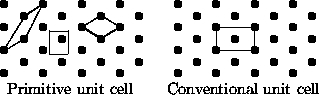
\includegraphics[scale=1.0]{img28}
\caption{Unit cells}
\label{hullpartlinje}
\end{figure}
\end{frame}

%\begin{frame}
%  The primitive unit cell contains only one lattice point, while the conventional contains more.
%
%\end{frame}
\section{Bravais lattices}

\begin{frame}
  There are collections of crystal classes which demand lattices of a given
  symmetry. 
  In three dimensions there are seven such systems.
\end{frame}

\begin{frame}
%  \begin{enumerate}
%	\item The cubic system
%	\item The triclinic system
%	\item The Monoclinic system
%	\item The orthorombic system
%	\item The trigonal system
%	\item The tetragonal system
%	\item The Hexagonal system
%  \end{enumerate}
  \begin{figure}[htp]
\centering
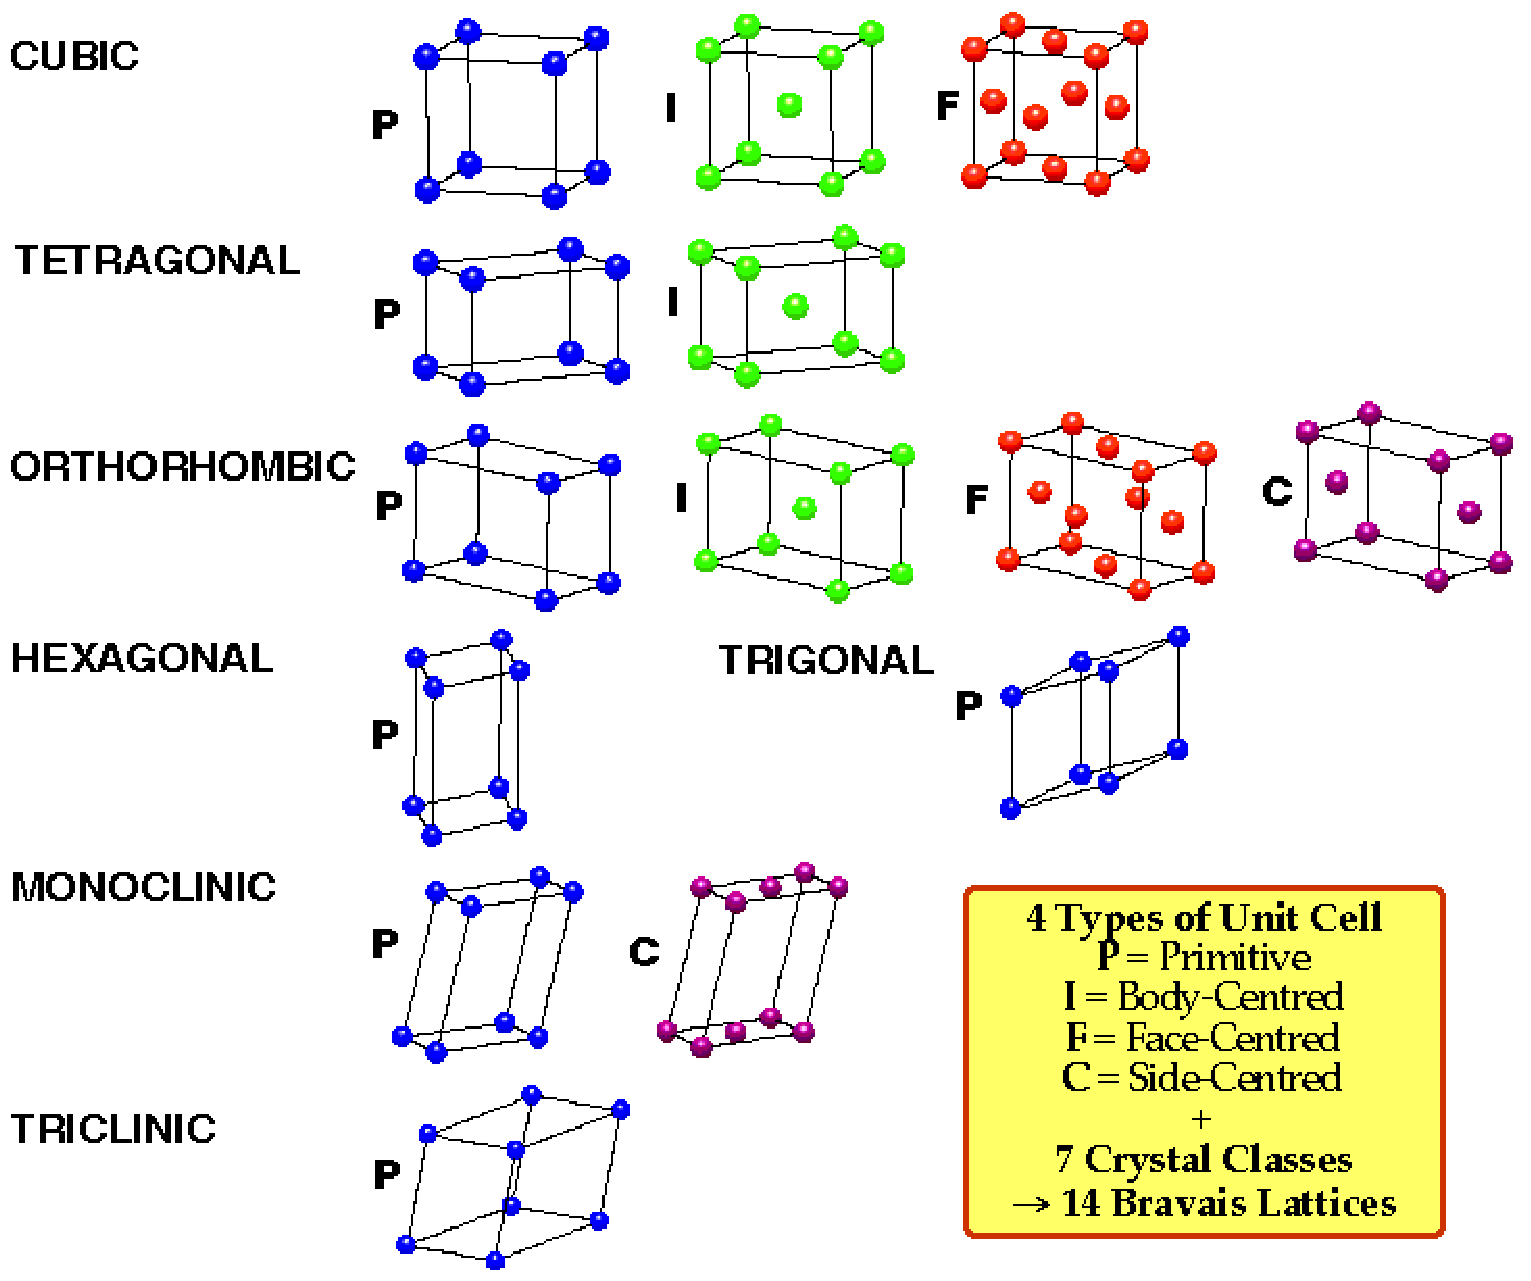
\includegraphics[scale=0.3]{Bravais}
\caption{The 14 different Bravais lattices and the 7 crystal systems.}
\label{fig:bravais}
\end{figure}

\end{frame}

\begin{frame} 
  The geometrical description of the crystal requires the specification 
  of the translation vectors $\mbf t_i$ as well as the 
  specification of the atom or ion positions within the cell: 
  $$\mbf d_1,~\mbf d_2\dots \mbf d_n.$$  
\end{frame}
\section{The reciprocal lattice}
\begin{frame}
  Beside the direct lattice in ordinary space described by the vectors 
  $$\mbf t_1,\mbf t_2~\mbox{and }\mbf t_3$$
  the reciprocal lattice in the dual space is also important, spanned by the 
  vectors
  $$\mbf g_1,~\mbf g_2~\mbox{and }\mbf g_3$$
  which again are defined by the relation 
  $$\mbf t_i \mbf g_j=2\pi\delta_{ij}.$$

\end{frame}

\section{The periodic Hamiltonian}
\begin{frame}
  The Hamiltonian 
  $$H=\frac{\mbf p^2}{2m}+v(\mbf r)$$
  is periodic in the potential
  $$v(\mbf r+\mbf R_n)=v(\mbf r).$$
  Thus it is possible to expand the potential in terms of the reciprocal
  vectors $\mbf G_m=m_1\mbf g_1+m_2\mbf g_2+m_3\mbf g_3$
  $$v(\mbf r)=\sum_mv(\mbf G_m)e^{i\mbf G_m\mbf r.}$$
\end{frame}

\begin{frame}
  The eigenfunctions to the Hamiltonian are the so called Bloch functions
  $$\psi_{\mu\mbf k}(\mbf r)=e^{i\mbf k\mbf r}u_{\mu\mbf k}(\mbf r),$$ where $u_{\mu\mbf k}(\mbf r)$ is periodic in $\mbf r$.
  We notice that:
  $$\psi_{\mu\mbf k}(\mbf r+\mbf R_n)=e^{i(\mbf k\mbf r+\mbf k\mbf R_n)}u_{\mu\mbf k}(\mbf r)=e^{i\mbf k\mbf R_n}\psi_{\mu\mbf k}(\mbf r)$$

  $$\int  \psi_{\mu \mbf k}(\mbf r)\psi_{\nu \mbf k'}(\mbf r)d\mbf r=\delta_{\mu\nu}\delta_{\mbf k \mbf k'}.$$

\end{frame}

\begin{frame}
  Inserting a Bloch function in the Schr\"odinger equation and eliminating the
  exponential from both sides yields the following equation
  \begin{equation*}
		  \left[\frac{1}{2}\left(-i\nabla+\mbf k\right)^2+V(\mbf r)\right]u_{\mu k}(\mbf r)=\varepsilon_{\mu}(\mbf k)u_{\mu k}(\mbf r)
  \end{equation*}
%  In general such an equation has an infinite set of of solutions 
%  $$\left(u_n(\mbf k,\mbf r),\varepsilon_{n,k}\right)$$
\end{frame}

\begin{frame}
    \begin{figure}[htp]
\centering
\includegraphics[scale=0.4]{BandStructure}
\caption{Band structure}
\label{fig:bands}
\end{figure}
\end{frame}


%\section{Hartree Fock with Bloch functions}
\begin{frame}
		The self consistent field equations, are solved for the $k$ values.
		\begin{equation*}
				F(k)C(k)=\varepsilon(k)S(k)C(k)
		\end{equation*}
  The Fock matrix, of the system, is given by
  \begin{equation}
	F_{ij}(k)=\sum_{R}e^{ikR}F_{i0,jR},
	   \label{hfbleq:totmatx2}
	 \end{equation}
	 where 
	 \begin{equation}
	   F_{i0jR}=T_{i0jR}+Z_{i0jR}+J_{i0jR}+X_{i0jR}.
	 \end{equation}
\end{frame}

%\begin{frame}
%  \begin{equation}
%	\begin{split}
%	  &T_{i0jR}=-\frac{1}{2m}\braopket{i0}{\nabla^2}{jR}\\
%	  &Z_{i0jR}=\sum_{R'}\braopket{i0}{\frac{Ze}{r-Z_{R'}}}{jR}\\
%	  &J_{i0JR}=\sum_{kR'}\braopket{i0kR'}{\frac{e^2}{|r_{12}}}{jRkR'}\\
%	  &X_{i0jR}=\sum_{kR'}\braopket{i0kR'}{\frac{e^2}{r_{12}}}{kR'jR}
%	\end{split}
%  \end{equation}
%\end{frame}

\section{Wannier functions}
\begin{frame}
  G.H. Wannier constructed functions which are orthogonal at different lattice sites, when computing electronic excitations levels in insulating crystals. 
  Wannier functions can be computed by a Fourier transform of the Bloch functions.
  $$w_{nR}(r)=\frac{1}{\sqrt \Omega}\int dke^{-ikR}\psi_n(k,r)$$
\end{frame}
\begin{frame}
  The orthogonality is easily verified
  \begin{equation}
	\begin{split}
			&\int w_{nR}(r)w_{n'R'}^*(r)dr=\frac{1}{\sqrt\Omega}\int dr\\
			&\times\int dke^{-ikR}\psi_n(k,r)\frac{1}{\sqrt \Omega}\int dk'e^{ik'R'}\psi_{n'}(k',r)\\
	&=\delta_{nn'}\frac{1}{\sqrt \Omega}\int dke^{-ik(R-R')}=\delta_{nn'}\delta_{RR'}.
	\end{split}
	\label{eq:orthoRR'}
  \end{equation}
\end{frame}
\section{Localized Wannier functions}
\begin{frame}
  A feature of Wannier functions is that they are in a sense localized.
  Roughly seen by the following integral:
  \begin{equation}
	  w_{n}(R_i-R)=\int d^3ku_{nk}(0)e^{ik(R_i-R)},
	    \label{waneq:decay}
	  \end{equation}
\end{frame}

\section{Non uniqueness of Wannier functions}
\begin{frame}
  Wannier functions are not unique, because of the freedom of choice of the
  phases of the Bloch orbitals as a function of wave vector $k$
  \begin{equation}
	\ket{\psi_{nk}}\rightarrow e^{i\theta_n(k)}\ket{\psi_{nk}}
  \end{equation}
  In case of degeneracy of bands, composite bands
  \begin{equation}
	\ket{\psi_{nk}}\rightarrow \sum_m U^k_{mn}\ket{\psi_{mk}}
  \end{equation}
\end{frame}

\begin{frame}
  The goal will be to pick out, from all the many arbitrary choices of Wannier
  functions, the particular set that is maximally localized according to some
  criterion.\\
  %The particular set of Wannier functions will, of course, remain arbitrary:
%  \begin{itemize}
%
%	\item There will always be an arbitrary overall phase of each of the $M$
%	  Wannier functions.
%
%	 \item There is a freedom to permute the $M$ Wannier functions among
%	   themselves.
%
%	 \item There is a gauge freedom to translate any one of the J Wannier
%	   functions by a lattice vector. That is, to decide which Wannier
%	   functions belong to the “home” unit cell labeled by site 0
%
%  \end{itemize}
  There are different methods for determining the ``maximally localized'' set of Wannier
  functions, like the minimization of the spread,
  \begin{equation}
	\Omega=\sum_n\left(\braopket{0n}{r^2}{0n}-|\braopket{0n}{r}{0n}|^2 \right), 
  \end{equation}
  of the Wannier functions in real space, which is performed by Marzari and Vanderbilt.

\end{frame}


%\begin{frame}
%\end{frame}


\section{Hartree Fock with Wannier functions}
\begin{frame}
A priori Wannier functions from Hartree-Fock:
Ansatz: Slater Determinant in terms of occupied Wannier orbitals, 
$w_{iR_j}(r_k),$
\[\Phi_0(r_{1},\cdots,r_{NM})=
  \begin{array}{|cccc|}
	w_{1R_1}(r_1) & w_{2R_1}(r_2) & \cdots & w_{NR_1}(r_{NM})\\
	w_{1R_2}(r_1) & w_{2R_2}(r_2)&\cdots&w_{NR_2}(r_{NM})\\
	\vdots & \vdots & \ddots & \vdots\\
	w_{1R_M}(r_{1}) & w_{2R_M}(r_{2}) & \cdots & w_{NR_M}(r_{NM})\\
  \end{array}
\]
\end{frame}



\begin{frame}
   \begin{equation*}
	\begin{split}
	  &E[\Phi_0(r_{1},\cdots,r_{NM})]=
	  \sum_{\mu R} \braopket{w_{\mu R}}{T+U}{w_{\mu R}}\\
	  &+\sum_{w_{\mu R}w_{\nu R'}}\Big(2\braopket{w_{\mu R}w_{\nu R'}}{v(r_{\mu\nu})}{w_{\nu R'}w_{\mu R}}\\
	  &-\braopket{(w_{\mu R}w_{\nu R'}}{v(r_{\mu\nu})}{w_{\mu R}w_{\nu R'}}\Big)
	\end{split}
  \end{equation*}
  is minimized with the condition $\braket{w_{\mu R}}{w_{\nu {R'}}}=\delta_{\mu\nu}\delta_{R R'}.$
 
\end{frame}

\begin{frame}
    The Wannier Hartree-Fock equation:
  \begin{equation*}
	\begin{split}
			&\hat{f}\ket{w_{\mu R}}=\sum_{\nu R'}\varepsilon_{\mu R\nu R'}\ket{w_{\nu R'}}\\
			&=\sum_{\nu}\varepsilon_{\mu R \nu R}\ket{w_{\nu R}}+\sum_{\substack{\nu \\R'\neq R}}\varepsilon_{\mu R \nu R'}\ket{w_{\nu R'}}
	\end{split}
  \end{equation*}
\end{frame}

\begin{frame}
		A new condition ($\braket{w_{\mu R}}{w_{\nu {R}}}=\delta_{\mu\nu}$) has usually been introduced where only intercell orthogonality
  is considered:
  \begin{equation*}
		  E[\Phi_0(r_{1},\cdots,r_{NM})]-\varepsilon_{\mu \nu}(\braket{w_{\mu R}}{w_{\nu {R}}}-\delta_{\mu\nu})
  \end{equation*}
  \begin{equation*}
		  V_{Orth}=\sum_{R}\sum_{\nu}\lambda^R_\nu
		  \ket{w_{\nu R}}\bra{w_{\nu R}}
  \end{equation*}
\end{frame}

\begin{frame}
		In our work we will stick to the condition $\braket{w_{\mu_R}}{w_{\nu_{R'}}}=\delta_{\mu\nu}\delta_{R R'}.$ The energy,
  \begin{equation*}
	\begin{split}
	  &E[\Phi_0(r_{1},\cdots,r_{NM})]=
	  \sum_{\mu_R} \braopket{w_{\mu_R}}{T+U}{w_{\mu_R}}\\
	  &+\sum_{\mu_R\nu_{R'}}\Big(2\braopket{w_{\mu_R}w_{\nu_{R'}}}{v(r_{\mu\nu})}{w_{\nu_{R'}}w_{\mu_R}}\\
	  &-\braopket{w_{\mu_R}w_{\nu_{R'}}}{v(r_{\mu\nu})}{w_{\mu_R}w_{\nu_{R'}}}\Big)
	\end{split}
  \end{equation*}
  will be minimized with the condition $\braket{w_{\mu_R}}{w_{\nu_{R'}}}=\delta_{\mu\nu}\delta_{R R'}.$
\end{frame}

\begin{frame}
  The Wannier Hartree-Fock equation becomes:
  \begin{equation*}
	\begin{split}
			\hat{f}\ket{w_{n_R}}=\sum_{\nu_{R'}}\varepsilon_{\mu_R\nu_{R'}}\ket{w_{\nu_{R'}}}
	\end{split}
  \end{equation*}
  where the Lagrangian multiplier ``matrix'' turns out to be hermitian $(\varepsilon_{\mu_R\nu_{R'}}=\varepsilon^*_{\nu_{R'}\mu_R})$.\\ It is possible to diagonalize the problem to an eigenvalue equation
  \begin{equation}
	\hat{f}\ket{w_{\mu_R}}=\varepsilon_{\mu_R}\ket{w_{\mu_R}}
  \end{equation}
\end{frame}

\section{Questions}
\begin{frame}
  \begin{itemize}
	\item Computational costs
	%\item How many unit cells contribute to the interactions
	\item Is the orthogonalizing potential necessary?
  \end{itemize}
\end{frame}


\end{document}
